\documentclass{iitsrc}
\usepackage{graphicx}
\usepackage{mflogo}
\usepackage{courier}
\usepackage[utf8]{inputenc}%some compilers use utf8x and need the prerendredUnicode characters
%\PrerenderUnicode{áäčďéíľĺňóôŕšťúýžÁÄČĎÉÍĽĹŇÓÔŔŠŤÚÝŽ}

% Please do not remove the following commands:
\editpages{1}{8}

\title{Stream analysis of incoming events using different data analysis methods\\~in Proceedings of IIT.SRC 2017}
\titlerunning{Stream analysis of incoming events using different data analysis methods in Proceedings of IIT.SRC 2017}
\author{Matúš}{Cimerman}
\supervision{\ms}
            {\infosys}
            {Dr. Jakub Ševcech}
            {\iiisse, \fiit}
\mail{matus.cimerman@gmail.com}
\field{To Be Added by Editor}

\begin{document}
\maketitle

\begin{multicols}{2}
\raggedcolumns

\begin{abstract}
Real-time stream processing and analysis experienced rapid interest gain across industries. Data analysis is an non-trivial task and gets even harder when it comes to streaming data analysis. Several constraints need to matched when analysing streams, e.g. usage of limited time and memory or real-time latency. In this work, we focus on ensemble tools aiming to ease data analysis process of changing streaming data for domain expert. Suppose domain expert doesn't have detail knowledge of standard process for data mining and analysis. In this work, we primarily target modelling and visualisation. With Hoeffding trees and classification task we evaluate our solution empirically and utilizing user study.
\end{abstract}

\section{Basics}
%
We do not hope to give you as extensive information as other sources (such
as~\cite{lamport:latex}). On Linux you can get fairly complete
information about \LaTeX{} commands via:
%
\begin{lstlisting}
    info latex
\end{lstlisting}
%
Here we only make few notes concerning obvious things you probably
already know.
%
You should properly divide your text into several sections (via
\verb|\section| and perhaps also \verb|\subsection| commands).
%
Do not change the font family and font sizes defined by the
\verb|iitsrc| class. These default values should be common for all
articles.
%
If you want to emphasize something (perhaps a newly introduced notion
or such), use the \verb|\em| command.
%
Usage of the bold face (the \verb|\bf| command) is very unusual in
normal \LaTeX{} text. It is not advised to use it explicitly.
%
End of a paragraph is indicated in the source code by an empty line.
%
You can use usual environments such as \verb|itemize| or
\verb|enumerate| to create bulleted or enumerated lists.
%
\section{Mathematical formul\ae, equations, figures and tables}
%
The \verb|equation| environment can be used for typesetting numbered
equations.
\begin{equation}
\label{eq:contestwinner}
e^{i\pi}+1=0
\end{equation}
It was produced with a following commands:
\begin{lstlisting}
   \begin{equation}
   e^{i\pi}+1=0
   \end{equation}
\end{lstlisting}
If you want later to refer to your equation, it is wise to accompany
your equation with a symbolic label, for example as below:
\begin{lstlisting}
   \begin{equation}
   \label{eq:contestwinner}
   e^{i\pi}+1=0
   \end{equation}
\end{lstlisting}
Now you can refer to it---the
Equation~\ref{eq:contestwinner}---by its
symbolical name rather than a concrete number. This is advantageous
because the order of equations might change over time. This reference
can be typeset as follows:
\begin{lstlisting}
   Equation~\ref{eq:contestwinner}
\end{lstlisting}
There is also \verb|equation*| environment which enables you to
typeset unnumbered equation.

There are also other useful \LaTeX{} commands and environments such as
\verb|eqnarray|. For example:
\begin{eqnarray}
x & \ll  & y_1 + \cdots + y_n\\
x & \leq & z
\end{eqnarray}
It enables you to put (non-)equalities nicely one below the other
pleasantly aligned. The above example was typeset by a following
command:
\begin{lstlisting}
   \begin{eqnarray}
   x & \ll  & y_1 + \cdots + y_n\\
   x & \leq & z
   \end{eqnarray}
\end{lstlisting}
%
If you need to typeset a table such as Table~\ref{tab:strategy} you can do it as follows:
%
\begin{table}[H]
\centering
    \caption{Specification of a strategy  $s(a)$ of agent $a$.}
    \label{tab:strategy}
        \begin{tabular}{|c|ccc|}
        \hline
        & penalty & penalty & movement\\
        & of agent $a$ & of agent $b$ & of agent $a$\\
        \hline
        1 & $p(a)=0$ & $p(b)=0$ & $S_1(a)$\\
        2 & $p(a)=0$ & $p(b)>0$ & $S_2(a)$\\
        3 & $p(a)>0$ & $p(b)=0$ & $S_3(a)$\\
        4 & $p(a)>0$ & $p(b)>0$ & $S_4(a)$\\
        \hline
    \end{tabular}
\end{table}
%
\begin{lstlisting}
    \begin{table}[H]
    \centering
        \caption{Specification of a strategy  $s(a)$ of agent $a$.}
        \label{tab:strategy}
            \begin{tabular}{|c|ccc|}
            \hline
            & penalty & penalty & movement\\
            & of agent $a$ & of agent $b$ & of agent $a$\\
            \hline
            1 & $p(a)=0$ & $p(b)=0$ & $S_1(a)$\\
            2 & $p(a)=0$ & $p(b)>0$ & $S_2(a)$\\
            3 & $p(a)>0$ & $p(b)=0$ & $S_3(a)$\\
            4 & $p(a)>0$ & $p(b)>0$ & $S_4(a)$\\
            \hline
        \end{tabular}
    \end{table}
\end{lstlisting}
%
If you need to use full-page tables, such as Table~\ref{tab:strategy2}, you can do this as follows:
\begin{table*}[bp]
\centering
    \caption{Please use full-page tables only if necessary.}
    \label{tab:strategy2}
        \begin{tabularx}{12.6cm}{|C|CCC|}
        \hline
        & penalty & penalty & movement\\
        & of agent $a$ & of agent $b$ & of agent $a$\\
        \hline
        1 & $p(a)=0$ & $p(b)=0$ & $S_1(a)$\\
        2 & $p(a)=0$ & $p(b)>0$ & $S_2(a)$\\
        3 & $p(a)>0$ & $p(b)=0$ & $S_3(a)$\\
        4 & $p(a)>0$ & $p(b)>0$ & $S_4(a)$\\
        \hline
    \end{tabularx}
\end{table*}
\begin{lstlisting}
  \begin{table*}[bp]
  \centering
      \caption{Please use full-page tables only if necessary.}
      \label{tab:strategy2}
          \begin{tabularx}{12.6cm}{|C|CCC|}
          \hline
          & penalty & penalty & movement\\
          & of agent $a$ & of agent $b$ & of agent $a$\\
          \hline
          1 & $p(a)=0$ & $p(b)=0$ & $S_1(a)$\\
          2 & $p(a)=0$ & $p(b)>0$ & $S_2(a)$\\
          3 & $p(a)>0$ & $p(b)=0$ & $S_3(a)$\\
          4 & $p(a)>0$ & $p(b)>0$ & $S_4(a)$\\
          \hline
      \end{tabularx}
  \end{table*}
\end{lstlisting}
If you need to include a figure to your document,
such as Figure~\ref{fig:fractaltree},
\begin{figure}[H]
    \begin{center}
        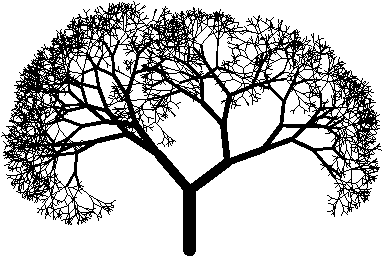
\includegraphics{tree}
        \caption{Sample output of a fractal tree drawing algorithm.}
        \label{fig:fractaltree}
    \end{center}
\end{figure}
\begin{figure*}[t]
    \begin{center}
        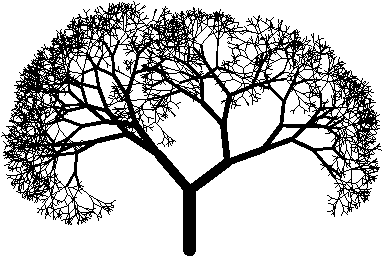
\includegraphics{tree}
        \caption{Please use full-page images only if necessary.}
        \label{fig:fractaltree2}
    \end{center}
\end{figure*}
you can do it as follows:
\begin{lstlisting}
    \begin{figure}[H]
    \begin{center}
        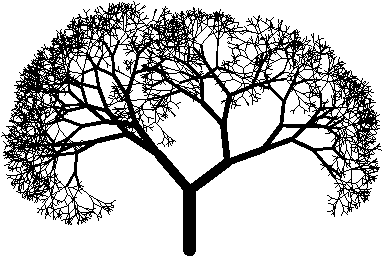
\includegraphics{tree}
        \caption{Sample output of a fractal tree drawing algorithm.}
          \label{fig:fractaltree}
      \end{center}
  \end{figure}
\end{lstlisting}
If you need to include a full-page figure to your document, such as Figure~\ref{fig:fractaltree2}, you can do it as follows:
\begin{lstlisting}
    \begin{figure*}[t]
        \begin{center}
            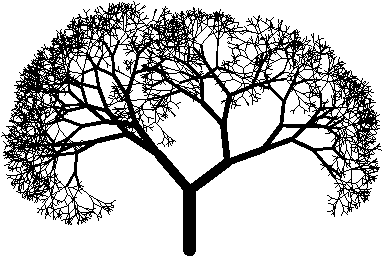
\includegraphics{tree}
            \caption{Please use full-page images only if necessary.}
            \label{fig:fractaltree2}
        \end{center}
    \end{figure*}
\end{lstlisting}
%
If you process your document with \LaTeX\ you will have to
provide all your figures as EPS (Encapsulated Postscript) files.
If you process your document with PDF\LaTeX\ you will have to
provide all your figures as PDF files. Several graphical programs
are able to export pictures to these two formats.
If possible, please use a
vector editor. Please do not convert bitmaps into EPS or PDF.
The printed results are then usually ugly.

Note that since you have given a figure a symbolic name (in this case
\verb|fig:fractaltree|), you can refer to this figure as follows:
\begin{lstlisting}
   Figure~\ref{fig:fractaltree}
\end{lstlisting}
This is advantageous because regardless of the fact how you reorder
your figures in the document, the references to them will never
break unless you change their symbolical name.
%
Do not forget to describe your figure with a \verb|\caption| command.
%
Due to technological constraints, included figures should be
\begin{itemize}
\item black-and-white,
\item minimal thickness of lines should be at least 0.25 mm,
\item do not use half-tones; use raster instead to express various
degrees of gray.
\end{itemize}
%
If you need to insert a pseudo code of an algorithm into the
paper, you can use the algorithms package for \LaTeX.
Documentation and example in \TeX{} file can be found in the zip
file available on
\url{http://texcatalogue.sarovar.org/entries/algorithms.html}.
%
Please do not refer to various parts
of your document via page numbers. Instead, give a symbolic name
to your sections (via \verb|\label| command) and refer to your
sections via \verb|\ref| command.
%
Please leave the \verb|\editpages| command from a ``minimal article
source code'' in place. Its
purpose is related to combining particular articles to a single volume
and if you delete it, someone will have later add it back. So if you
leave it where it is, you will save yours someone else's time.
%
\section{The bibliography}
%

\def\BibTeX{{\rmfamily B\kern-.05em%
    \textsc{i\kern-.025em b}\kern-.08em%
    T\kern-.1667em\lower.7ex\hbox{E}\kern-.125emX}}

\LaTeX{} document usually creates bibliography references via \BibTeX.
Basic information about \BibTeX{} is in~\cite{lamport:latex}. You are
encouraged to use it too. Bibliography references are usually inserted
in the document as follows:
\begin{lstlisting}
   \bibliography{common}
   \bibliographystyle{iitsrc}
\end{lstlisting}
Be sure to use the \verb|iitsrc| style as suggested above. We used \BibTeX{}
also for typesetting bibliographic references cited within this
document. So you can look at the source code ({\tt demo.tex}) and the
compilation instructions ({\tt Makefile}) to see how it was
generated. The {\tt common.bib} file contains the bibligraphy resources
we collected over time. There are various entries in the form:
\begin{lstlisting}
    @ARTICLE{OwickiGries76b,
        AUTHOR = {S. Owicki and D. Gries},
        TITLE = "Verifying Properties of Parallel Programs,
                 an axiomatic approach",
        JOURNAL = cacm,
        VOLUME = 19,
        NUMBER = 5,
        PAGES = {279-285},
        MONTH = may,
        YEAR = 1976
    }
\end{lstlisting}
Each such entry contains logical information about the particular source
of information. You can add your sources of information therein. Some
information about how to do that can be found in~\cite{lamport:latex}
(Appendix B).  \BibTeX{} finds out which ones you cite within your
document and format the data it finds in your {\tt *.bib} (in this case
{\tt common.bib}) file according to the instructions in the {\tt *.bst}
(in this case {\tt iitsrc.bst}) file. All you have to do within your
document is to \verb|\cite{key}| them.

Other example citated
sources:~\cite{CHS03RR,friedman:switching,henessy:computer,henrio:thesis,MannaPnueli82,MisraChandy,OwickiGries76b,vardhan98distributed,WidomPanangaden,C99-draft,czarnecki:generative-programming,SWIG,leiserson:network}
%
\begin{itemize}
\item Item 1
\item Item 2
    \begin{itemize}
    \item Item 2.1
        \begin{itemize}
        \item Item 2.1.1
        \item Item 2.1.2
        \item Item 2.1.3
        \end{itemize}
    \end{itemize}
\item Item 3
\end{itemize}
%
A numbered list should be formatted as follows:
%
\begin{enumerate}
\item Item
    \begin{enumerate}
    \item Item
        \begin{enumerate}
        \item Item
        \end{enumerate}
    \end{enumerate}
\end{enumerate}
%
\acknowledgement{Here you should mention the names of grants
                 which funded the work on this article. As defined
                 by the particular grant.}


% Please do not remove this.
\let\OLDthebibliography\thebibliography
\renewcommand\thebibliography[1]{
  \OLDthebibliography{#1}
  \setlength{\parskip}{5pt}
 \footnotesize
}

\bibliography{common}
\bibliographystyle{iitsrc}

\end{multicols}
\end{document}
